\documentclass[times, utf8, diplomski]{fer}
\usepackage{booktabs}
\usepackage{cite}
\usepackage{graphicx}
\usepackage{xcolor}
\usepackage[]{algorithm2e}

\graphicspath{ {./img/} }

% Math
\def\mat#1{\underline{#1}}
\def\expect{\mathbb{E}}
\def\pfrac#1#2{\frac{\partial #1}{\partial #2}}
\def\dfrac#1#2{\frac{d #1}{d #2}}

% TODO notes
\def\TODO#1{\noindent\textcolor{red}{TODO: \textit{#1}}\newline}
\def\todo#1{\TODO{#1}}
\def\todoimg#1{\begin{center} \textcolor{red}{IMAGE: \textit{#1}} \end{center}}

\begin{document}

\thesisnumber{1966}

\title{Optimizirane izlazne funkcije klasifikatora temeljenog na umjetnim neuronskim mrežama u domeni implementacijskih napada na kriptografske uređaje}

\author{Juraj Fulir}

\maketitle

% Ispis stranice s napomenom o umetanju izvornika rada. Uklonite naredbu \izvornik ako želite izbaciti tu stranicu.
\izvornik

\zahvala{ZAHVALA'n'STUFF}

\tableofcontents

\chapter{Uvod}
\todo{ Opis problema }

\chapter{Implementacijski napadi na kriptografske uređaje}

\section{Side-channel napadi}
\todo{ Postoji nekoliko vrsta.}
\todo{ Ovdje se obrađuje DPA.}

\section{Izvedba napada}
\todo{ Uštekaj uređaj, osciloskop na to i to mjesto i snimaj}
\todo{ Provjeri mogućnosti i zaključi najvjerojatniju}
\todo{ Problem netraktabilnosti postupka -> neuralke <3}

\section{DPA skupovi podataka}
\todo{Tko i cilj*}
\todo{Ne zaboravi referencu na stranicu!}

\subsection{DPAv2}
\todo{Kada je napravljen i ko ga je radil}
\todo{Jel HW ili onaj pravi}
\todoimg{PCA redukcija iz jn}
\todoimg{Statistike iz jn}
\todo{Mjere dobrote klasifikacije}

\subsection{DPAv4}
\todo{Kada je napravljen i ko ga je radil}
\todo{Jel HW ili onaj pravi}
\todoimg{PCA redukcija iz jn}
\todoimg{Statistike iz jn}
\todo{Mjere dobrote klasifikacije}

\chapter{Klasifikator temeljen na umjetnim neuronskim mrežama}

\section{Umjetne neuronske mreže}
Umjetne neuronske mreže (nadalje „neuronske mreže“) koristimo za modeliranje višedimenzijske funkcije ili distribucije kojom se aproksimira rješenje zadanog problema iz konačnog broja primjera. Vrlo su moćan alat za savladavanje teških zadataka u raznim područjima, često dostižući ljudske performanse na zadanom problemu. Danas su vrlo raširene u raznim područjima od kojih su samo neka: računalni vid \citep{alexnet,yolo}, prirodna obrada jezika \citep{word2vec,char_cnn} i podržano učenje \citep{atari,active_learn}.

\subsection{Građa}
Neuronske mreže građene su od međusobno povezanih jedinica, tzv. neurona, modeliranih prema pojednostavljenom modelu biološkog neurona. Neuron očitava ulazne značajke sustava ili izlaze drugih neurona te ažurira svoje unutarnje stanje (aktivaciju) i stvara odziv (izlaz). Utjecaj ulaza na neuron vrednuje se težinama \engl{weights} koje definiraju kako se neuron ponaša u ovisnosti o pojedinim ulazima. Aktivacijski prag neurona \engl{bias} određuje jedinstvenu osjetljivost neurona na jačinu podražaja. Težine i prag neurona nazivamo parametrima neurona.

\todo{Što sve biolozi vele o neuronima? https://www.ncbi.nlm.nih.gov/pmc/articles/PMC3812748/}

\begin{figure}[h]
\centering
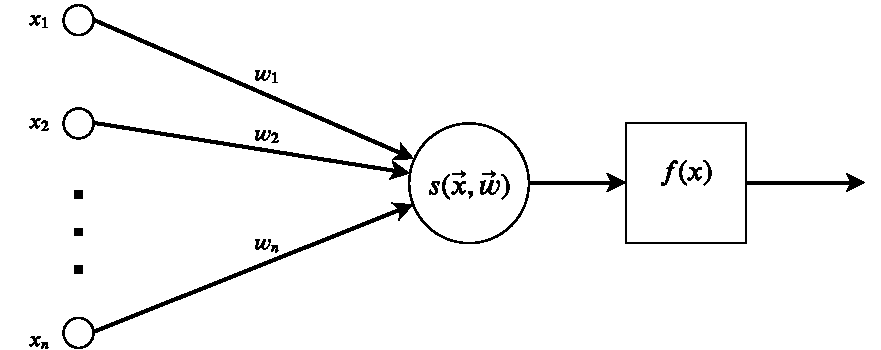
\includegraphics[scale=0.7]{Neuron.pdf}
\caption{Prikazani osnovni dijelovi neurona su težine dendrita ($w_i$), aktivacijska funkcija ($a(\vec{x},\vec{w})$) i izlazna funkcija ($f(x)$). Prag neurona nije prikazan zbog jednostavnosti dijagrama.}
\label{fig:neuron}
\end{figure}

Način na koji iz ulaza gradimo unutarnje stanje (aktivaciju) neurona opisujemo aktivacijskom funkcijom. Najpopularnije aktivacijske funkcije jesu afina funkcija i unakrsna korelacija.
Afina funkcija je skalarni produkt vektora ulaza s vektorom težina neurona uz dodatak vrijednosti praga. Parametri neurona definiraju nagib i pomak ravnine u prostoru ulaza koja opisuje aktivaciju neurona. Primijenjuje se kada se ulazi u model mogu zapisati vektorom značajki čiji raspored nije bitan.
\begin{equation}
f(\vec{x};\mat{W},\vec{b})=\mat{W}^T \cdot \vec{x} + \vec{b}
\end{equation}

\todo{Spomeni distance based aktivacije (ANFIS?)}
\todo{Spomeni i složenije metode: \citep{network_in_network}}

Pretvorbu aktivacije neurona u izlazni signal opisujemo izlaznom funkcijom koja se detaljnije obrađuje u poglavlju \ref{sec:izlazne_fje}. Aktivacijska i izlazna funkcija definiraju prijenosnu funkciju koja ujedno opisuje ponašanje cijelog neurona \citep{function_survey}. U praksi se pojam aktivacijske i prijenosne vrlo često ekvivalentno koristi na mjestu pojma izlazne funkcije, no ovaj rad se drži prethodno navedene i jasnije notacije.
\begin{equation}
t(x) = (f \circ a)(x) = f(a(x))
\end{equation}

Povezivanjem neurona gradi se arhitektura mreže koja određuje kako podatci i gradijenti teku kroz mrežu, a time utječu na brzinu učenja i inferencije neuronske mreže. Najčešće se koriste slojevite unaprijedne arhitekture zbog jednostavnosti izvedbe. Unaprijedne arhitekture propuštaju podatke samo u jednom smjeru odnosno već izračunati neuroni se ne izračunavaju ponovno, što je posebno pogodno za optimizaciju širenjem unatrag, detaljnije opisanu u poglavlju \ref{sec:backprop}. Slojevite arhitekture omogućuju paralelizaciju izvođenja operacija na grafičkim karticama što značajno ubrzava postupke učenja i inferencije. Pri definiciji slojevite arhitekture najčešće je dovoljno navesti samo redoslijed slojeva, no ponekad je potrebno definirati i način povezivanja slojeva npr. pri uporabi preskočnih veza \citep{highwaynet, resnet, densenet}. Prvi sloj služi za postavljanje ulaza mreže i nazivamo ga ulaznim slojem mreže. Posljednji sloj mreže služi nam za ekstrakciju izlaza te mjerenje kakvoće mreže i nazivamo ga izlaznim slojem mreže. Svi slojevi između ulaznog i izlaznog sloja nazivaju se skrivenim slojevima.

Potpuno povezana arhitektura je najjednostavnija arhitektura za zadatak klasifikacije. Svaki neuron u potpuno povezanom sloju aktivira se pomoću svih izlaza iz prethodnog sloja. Za naučeni potpuno povezani sloj kažemo da vrši ekstrakciju značajki iz svojih ulaza. Geometrijski gledano, svaki neuron vrši mapiranje značajki iz dimenzije prethodnog sloja u novu dimenziju s ciljem modeliranja boljih značajki.

\todo{Daj neki dokaz za ovo gore.}

Unakrsna korelacija, za razliku od afine funkcije, koristi informaciju o susjednosti ulaznih značajki. Ulaz za takav model je definiran n-dimenzijskim tenzorom, a neuron uzima samo jedan pod-tenzor ulaza (vidljiva regija) i nad njime računa skalarni produkt s n-dimenzijskim tenzorom parametara (jezgrom). Kada su ulazi slike u boji ulazni tenzor ima 3 dimenzije (visina, širina, RGB kanali) pa stoga i jezgra ima 3 dimenzije, no znantno manje visine i širine. Unakrsna korelacija prozvana je konvolucijom jer radi na istom principu, a jedina razlika je da se elementi jezgre indeksiraju zrcaljeno po obje osi. S obzirom da se parametri jezgre uče automatski, nije nam bitno definirati orijentaciju jezgre.
\begin{equation}
f(\mat{X};\mat{W})=\mat{X} \circledast \mat{W}
\end{equation}

\todo{Je li uopće potrebno spominjat konvoluciju?}
\todo{Raspisat konvoluciju po elementima?}

\subsection{Optimizacija umjetne neuronske mreže}
Optimizacijom parametara neuronska mreža prilagođava se danom zadatku, odnosno kažemo da mreža 'uči'. Optimizaciju parametara najčešće izvodimo gradijentnim spustom, uz pretpostavku derivabilnosti svih komponenata neuronske mreže. Kada ta pretpostavka ne vrijedi koriste se algoritmi kombinatorne optimizacije poput evolucijskih algoritama. U ovom radu optimizacija se vrši gradijentnim spustom.

\subsubsection{Gradijentni spust}

\todoimg{gradijentni spust unimodalna vs višemodalna (gdje preskoći brdo i uleti u bolji optimum)}
\label{fig:gradientni_spust}

Gradijentni spust je algoritam pronalaska minimuma funkcije vođen gradijentom te funkcije. Za zadanu početnu točku iterativno se pomiče u smjeru suprotnom od gradijenta funkcije u toj točki dok ne zadovolji neki od uvijeta zaustavljanja. Na strmim funkcijama gradijent je često prevelik i može izazvati oscilaciju ili divergenciju (slika \ref{fig:oscilira_divergira}). Stoga se gradijent pri pomaku skalira s koeficijentom pomaka $\mu$. Dobro odabran koeficijent pomaka može osigurati bržu konvergenciju, a kod višemodalnih funkcija i pronalazak boljeg optimuma (slika \ref{fig:gradientni_spust}).

\todo{spomeni negdje da generalno ne znamo koji je globalni optimum}

\begin{algorithm}[H]
\KwData{funkcija $f(x)$}
\KwData{koeficijent pomaka $\mu$}
\KwData{početna točka $x_0$}
\KwResult{optimalna točka $x^*$}
\For{uvijet nije zadovoljen}
aaa
\EndFor
\caption{Gradijentni spust}
\label{alg:grad_spust}
\end{algorithm}


Početna točka utječe na ishod algoritma. Kod višemodalnih funkcija s optimumima različitih kvaliteta, početna točka može definirati u koji će lokalni optimum algoritam konvergirati (slika \ref{fig:pocetna_tocka}). 

\todoimg{graidjentni spust stope spuštanja (velka, mala, taman)}
\label{fig:oscilira_divergira}

Broj iteracija definira koliko se puta pomičemo iz početne točke, što definira i trajanje algoritma. Generalno želimo skratiti vrijeme pretraživanja te povećati koeficijent spusta kako bismo koristili manje pomaka. No u praksi najčešće nailazimo na višemodalne funkcije sa strmim regijama koje izazivaju oscilacije i mogu izazvati divergenciju. Stoga se češće koriste manji pomaci kroz više iteracija. Dodatno se mogu dodati modifikacije gradijenta koje nude ograničavaju veličinu gradijenta (odsijecanje gradijenta i sl.).

\todoimg{gradijentni spust sa početnim točkama (jedna ode u lok, jedna ode u glob, jedna zapne desno na platou)}
\label{fig:pocetna_tocka}

Problem se javlja ako algoritam "odluta" u visoravan na kojoj su gradijenti vrlo mali, a sama regija je s obzirom na pomake ogromna (slika \ref{fig:pocetna_tocka}). Kad gradijent postane neupotrebljivo malen kažemo da je "\textit{iščeznuo}". U takvim slučajevima pomaže dodavanje momenta koji se akumulira kroz više iteracija i dodaje vektoru gradijenta. Kad algoritam naiđe na regiju s vrlo malim gradijentima, moment pokušava izvuči algoritam iz visoravni pomičući ga u smjeru koji je akumuliran. Kako moment ne bi izvukao algoritam iz optimuma, dodaje mu se koeficijent "\textit{zaboravljanja}" kojim se stari vektor momenta djelomično zaboravlja u korist novog vektora pomaka (jednadžba \ref{eq:moment_update}). Moment može pomoći i pri zaobilaženju lokalnih optimuma (slika \ref{fig:pocetna_tocka}).

\begin{equation}
\label{eq:moment_update}
\begin{split}
v \gets \alpha \cdot v - \mu \cdot g \\
x \gets x + v
\end{split}
\end{equation}

\todoimg{moment prije i na visoravni, moment za savladavanje brda}
\label{fig:visoravan}

Algoritam je primijenjiv na funkcije proizvoljne dimenzionalnosti uz pretpostavku derivabilnosti u svakoj točki. Za proizvoljnu realnu funkciju, uz dobro odabrane hiperparametre, algoritam će konvergirati u jedan od lokalnih optimuma, no algoritam generalno nema garanciju konvergencije u globalni optimum. Garanciju pronalaska globalnog optimuma nudi jedino za unimodalne funkcije uz odgovarajuće hiperparametre algoritma (slika \ref{fig:gradientni_spust}).

\subsubsection{Funkcija gubitka}
Pri učenju umjetnih neuronskih mreža potrebno je definirati funkciju gubitka. Funkcija gubitka, za dani ulaz, uspoređuje predikciju mreže sa željenim vrijednostima te dodjeljuja magnitudu pogreške (realan broj). Funkciju gubitka potrebno je pažljivo odabrati jer ona definira što je ishod učenja te utječe na učenje svakog parametra (kao što je opisano u poglavlju \ref{sec:backprop}). Funkcija gubitka često je usko vezana uz vrstu problema koji se rješava i izlaznu funkciju posljednjeg sloja neuronske mreže.

\todo{oba imaju neg.log.izglednost, no pretpostavljaju razl. distribucije da dobiješ kvadratni ili ovaj drugi loss}

U problemima regresije, najčešće se koristi funkcija kvadratnog gubitka koja računa odstupanje izlaza neuronske mreže od željenih vrijednosti. Uz ovaj gubitak najčešće se koristi funkcija identiteta u izlaznom sloju. Ova funkcija je brza i jednostavna
\begin{equation}
L(\theta) = \frac{1}{N} \sum_{(\vec{x},\vec{y})\in (X,Y)} \sum_{i}^{|\vec{y}|} (f(\vec{x};\theta)_i - \vec{y}_i)^2
\end{equation}

U problemima klasifikacije, koristi se funkcija negativne logaritamske izglednosti. 
\begin{equation}
L(\theta) = -\expect ...
\end{equation}

\subsubsection{Optimizacija širenjem unatrag}
\label{sec:backprop}
Funkcija gubitka opisuje pogrešku čitave mreže te ovisi o svakom ugodljivom parametru mreže. Takva formulacija problema omogućuje nam da svaki parametrar mreže ugađamo gradijentnim spustom. Dakle, za parametriziranu funkciju $f(x;\theta)$ tražimo one parametre $\theta^*$ za koje je gubitak najmanji na danim parovima ulaznih i izlaznih podataka.
\begin{equation}
\theta^* = argmin_\theta L(x,y; \theta), \quad \forall (x,y) \in (X,Y)
\end{equation}

S obzirom da se mreža sastoji od ulančanih nelinearnih neurona s parametrima, gubitak moramo proslijediti sekvencijalno širenjem unazad (prema ulazima u mrežu). Pri tome koristi se pravilo ulančavanja parcijalne derivacije kompozicije funkcija.
\begin{equation}
\dfrac{}{x} f(g(x)) = \pfrac{f(g(x))}{g(x)} \cdot \pfrac{g(x)}{x}
\end{equation}

Pojedini neuron je parametrizirana funkcija i može se prikazati grafom. Vidimo da se ulazni gradijent prolaskom kroz neuron širi na ostale elemente i na ulaze neurona koji vode do prethodnih neurona. Primijetimo i da se širi u suprotnom smjeru od podatkovnog toka. Iz toga proizlazi naziv "\textit{širenjem unazad}".

\todoimg{neuron kao graf + tok gradijenata}
\label{fig:neuron_grad}

Želimo li učiti mrežu gradijentnim spustom, svaki parametar mreže treba imati pristup gradijentu. S obzirom da je neuron parametrizirana funkcija, kojom ulančavanjem gradimo mrežu, dovoljno je pokazati da pojedini neuron osigurava svojim parametrima pristup gradijentu te da gradijent šalje svojim prethodnicima s kojima je povezan. Na slici \ref{fig:neuron_grad} vidimo da je to ostvarivo, što dokazuju i formule:
\begin{align}
\begin{split}
\pfrac{L(x,y;\theta)}{s(x;w)} &= \pfrac{L(x,y;\theta)}{o(x;w)} \cdot \pfrac{o(x;w)}{s(x;w)} \\
&= \pfrac{L(x,y;\theta)}{o(x;w)} \cdot f'(x)
\end{split}
\end{align}

\begin{align}
\begin{split}
\pfrac{L(x,y;\theta)}{x_i} &= \pfrac{L(x,y;\theta)}{s(x;w)} \cdot \pfrac{s(x;w)}{x_i} \\
&= \pfrac{L(x,y;\theta)}{o(x;w)} \cdot f'(x) \cdot w_i
\end{split}
\end{align}

\begin{align} \label{eq:w_update}
\begin{split}
\pfrac{L(x,y;\theta)}{w_i} &= \pfrac{L(x,y;\theta)}{s(x;w)} \cdot \pfrac{s(x;w)}{w_i} \\
&= \pfrac{L(x,y;\theta)}{o(x;w)} \cdot f'(x) \cdot x_i
\end{split}
\end{align}

\begin{align}
\begin{split}
\pfrac{L(x,y;\theta)}{w_0} &= \pfrac{L(x,y;\theta)}{s(x;w)} \cdot \pfrac{s(x;w)}{w_0} \\
&= \pfrac{L(x,y;\theta)}{o(x;w)} \cdot f'(x) \cdot 1
\end{split}
\end{align}

\subsubsection{Stohastički gradijentni spust}

\subsubsection{Optimizator}
Gradijentni spust (algoritam \ref{alg:grad_spust}) 

\todo{uporaba momenta i momenta na kvadrat (interpretacija)}
\todo{Adam}

\subsubsection{Inicijalizacija parametara}
Inicijalizacija parametara mreže je sinonim za odabir početne točke pri gradijentnom spustu.

\todo{važnost dobre inicijalizacije}
\todo{Xavier}

\subsubsection{Regularizacija}
\todo{geometrijski opis deciziske granice}
\todo{podnaučena, generalizira, prenaučena}
\todoimg{podnaučena, generalizira, prenaučena}
\todo{L1}
\todo{L2}
\todo{Spomeni pokoju još}

\subsection{Svojstva}
\todo{kompresija}
\todo{generalizacija}
\todo{univerzalna aproksimacija}

\subsection{Problemi}
\todo{Problem odabira arhitekture, aktivacijske funkcije i hiperparametara}
\todo{Problem pretreniranosti + neprijateljski primjeri}

Arhitektura, prijenosne funkcije i parametri definiraju neuronsku mrežu te njihov odabir značajno utjeće na performanse neuronske mreže. Učenje 

Derivabilne neuronske mreže optimiziraju se optimizatorom koji određuje kako se mijenjaju parametri. Za ugađanje parametara najčešće se koristi gradijentni spust, uz pretpostavku derivabilnosti čitave neuronske mreže. Kada pretpostavka ne vrijedi najčešće se koriste evolucijski algoritmi.

\section{Izlazne funkcije}
\label{sec:izlazne_fje}
\todo{Bitka za odabir izlazne fje (nađi onaj rad di pljuje po sigmoidi i relu (elu rad?))}
\todo{Usporedbe funkcije i derivacije}
\todo{Navedene su funkcije koje su razmatrane}

\subsection{Funkcija identiteta}
\engl{Identity function}

\todo{Dokaz da cijela mreža postaje linearna}

\subsection*{Ispravljena linearna jedinica (ReLU)}
\engl{Rectified linear unit}

\todo{bez i sa cutoff}

\begin{equation}
\begin{split}
f(x) = 
\begin{cases}
x,		& \text{ako } x > 0 \\
0,		& \text{inače}
\end{cases}
\end{split}
\qquad
\begin{split}
f'(x) = 
\begin{cases}
1,		& \text{ako } x > 0 \\
0,		& \text{inače}
\end{cases}
\end{split}
\end{equation}

\subsection*{Propusna ispravljena linearna jedinica (LReLU)}
\engl{Leaky ReLU}

\begin{equation}
\begin{split}
f(x) = 
\begin{cases}
x,			& \text{ako } x > 0 \\
\alpha x,	& \text{inače}
\end{cases}
\end{split}
\qquad
\begin{split}
f'(x) = 
\begin{cases}
1,		& \text{ako } x > 0 \\
\alpha,	& \text{inače}
\end{cases}
\end{split}
\end{equation}

\subsection*{Ispravljena linearna jedinica s pragom (ThReLU)}
\engl{Thresholded ReLU}

\begin{equation}
\begin{split}
f(x) = 
\begin{cases}
x,		& \text{ako } x > \theta \\
0,		& \text{inače}
\end{cases}
\end{split}
\qquad
\begin{split}
f'(x) = 
\begin{cases}
1,		& \text{ako } x > \theta \\
0,		& \text{inače}
\end{cases}
\end{split}
\end{equation}

\subsection*{(RReLU)}
\engl{Randomized leaky ReLU}

\subsection*{Eksponencijalno-linearna jedinica (ELU)}
\engl{Exponential linear unit}

\begin{equation}
\begin{split}
f(x) = 
\begin{cases}
x,					& \text{ako } x > 0 \\
\alpha (e^x - 1),	&  \text{inače}
\end{cases}
\end{split}
\qquad
\begin{split}
f'(x) = 
\begin{cases}
1,	 		& \text{ako } x > 0 \\
\alpha e^x,	& \text{inače}
\end{cases}
\end{split}
\end{equation}

\subsection*{Skalirana eksponencijalno-linearna jedinica (SELU)}
\engl{Scaled exponential linear unit}

\begin{equation}
\begin{split}
f(x) = \lambda
\begin{cases}
x,					& \text{ako } x > 0 \\
\alpha (e^x - 1),	&  \text{inače}
\end{cases}
\end{split}
\qquad
\begin{split}
f'(x) = \lambda
\begin{cases}
1,	 		& \text{ako } x > 0 \\
\alpha e^x,	& \text{inače}
\end{cases}
\end{split}
\end{equation}

\subsection*{(GELU)}
\engl{Gaussian error linear unit}

\subsection*{Sigmoida ($\sigma $)}
\engl{Sigmoid}

\begin{equation}
\begin{split}
f(x) = \frac{1}{1+e^{-x}}
\end{split}
\qquad
\begin{split}
f'(x) = \sigma(x)(1-\sigma(x))
\end{split}
\end{equation}

\subsection*{Tvrda sigmoida}
\engl{Hard sigmoid}

\begin{equation}
\begin{split}
f(x) = min(1,\ max(0,\ 0.2x + 0.5))
\end{split}
\qquad
\begin{split}
f'(x) = 
\begin{cases}
0.2,	 		& \text{ako } x \in [-2.5, 2.5] \\
0,	& \text{inače}
\end{cases}
\end{split}
\end{equation}

\subsection*{Swish}
\begin{equation}
\begin{split}
f(x) = x \sigma(\beta x)
\end{split}
\qquad
\begin{split}
f'(x) &= \sigma(\beta x) + \beta x \cdot \sigma(\beta x)(1-\sigma(\beta x)) \\
&= \frac{e^x \cdot (e^x + x + 1)}{(e^x + 1)^2}
\end{split}
\end{equation}

\subsection*{Tangens hiperbolni (tanh)}

\begin{equation}
\begin{split}
f(x) = \frac{e^x - e^{-x}}{e^x + e^{-x}}
\end{split}
\qquad
\begin{split}
f'(x) = 1 - tanh^2(x)
\end{split}
\end{equation}

\subsection*{Tvrdi tangens hiperbolni}
\engl{Hard tanh}

\begin{equation}
\begin{split}
f(x) =
\begin{cases}
-1,	 		& \text{ako } x < 1 \\
x,	 		& \text{ako } x \in [-1,1] \\
1,	& \text{inače}
\end{cases}
\end{split}
\qquad
\begin{split}
f'(x) =
\begin{cases}
0,	 		& \text{ako } x < 1 \\
1,	 		& \text{ako } x \in [-1,1] \\
0,	& \text{inače}
\end{cases}
\end{split}
\end{equation}

\subsection*{Racionalna aproksimacija tanh}
\engl{Rational tanh}

\todo{DL4J ima bug u derivaciji ove fje}

\begin{equation}
f(x) = 1.7159 \cdot tanh(\frac{2}{3}x)\text{,\quad gdje }
tanh(x) \approx sgn(x)(1 - \frac{1}{1 + |x| + x^2 + 1.41645 \cdot x^4}) \\
f'(x) =
\end{equation}

\subsection*{Ispravljeni tanh}
\engl{Rectified tanh}

\subsection*{Softmax}
\begin{equation}
\begin{split}
f(\vec{x}) = \frac{e^{\vec{x}}}{\sum_ie^{\vec{x_i}}}
\end{split}
\qquad
\begin{split}
f'(x) = \frac{e^x}{1+e^x}
\end{split}
\end{equation}

\subsection*{Softplus}
\begin{equation}
\begin{split}
f(x) = log(1+e^x)
\end{split}
\qquad
\begin{split}
f'(x) = \frac{e^x}{1+e^x}
\end{split}
\end{equation}

\subsection*{Softsign}
\begin{equation}
\begin{split}
f(x) = \frac{x}{1+|x|}
\end{split}
\qquad
\begin{split}
f'(x) = \frac{1}{(1+|x|)^2}
\end{split}
\end{equation}

\subsection*{Sinus (sin)}
\begin{equation}
\begin{split}
f(x) = sin(x)
\end{split}
\qquad
\begin{split}
f'(x) = cos(x)
\end{split}
\end{equation}

\subsection*{Kosinus (cos)}
\begin{equation}
\begin{split}
f(x) = cos(x)
\end{split}
\qquad
\begin{split}
f'(x) = -sin(x)
\end{split}
\end{equation}

\subsection*{Parabola $x^2$}
\begin{equation}
\begin{split}
f(x) = x^2
\end{split}
\qquad
\begin{split}
f'(x) = 2x
\end{split}
\end{equation}

\subsection*{Kubna parabola $x^3$}
\begin{equation}
\begin{split}
f(x) = x^3
\end{split}
\qquad
\begin{split}
f'(x) = 3x^2
\end{split}
\end{equation}

\subsection*{Gauss}
\begin{equation}
\begin{split}
f(x) = e^{-x^2}
\end{split}
\qquad
\begin{split}
f'(x) = -2x \cdot f(x)
\end{split}
\end{equation}

\chapter{Optimizacija simboličkom regresijom (tehnički genetskim programiranjem...)}

\section{Simbolička regresija}
* Opis i svojstva SR
* Utjecaj i brojnost parametara u GA (moš linkat i svoj završni rad :P)

\section{Taboo evolucijski algoritam}
* Problem konvergencije i stohastičnosti GP-a
* EA oplemenjen taboo listom iz algoritma Taboo pretraživanja

\section{Korišteni čvorovi i operatori (prostor pretraživanja)}
* Popis čvorova
* Popis operatora (un/bin)

\chapter{Implementacija}
???

\chapter{Rezultati}

\section{9class}

\subsection{Uobičajene izlazne funkcije}
* Opis postupka pretrage
* Tablica
* Komentar

\subsection{Utjecaj parametra veličine taboo liste}
* Tablica
* Komentar

\section{256class}

\subsection{Uobičajene izlazne funkcije}
* Opis postupka pretrage
* Tablica
* Komentar

\subsection{Utjecaj parametra veličine taboo liste}
* Tablica
* Komentar

\chapter{Buduća istraživanja}
* Primjena CNN na vremenskim uzorcima po uzoru na onaj rad
* Ispitivanje učinkovitosti korištene optimizacije na ostalim problemima
* Paralelna evolucija arhitekture i aktivacijskih fja

\chapter{Zaključak}
* Radi/Ne radi. 
* Pronađene zanimljivosti. 
* Pouka za doma.

\bibliography{literatura}
\bibliographystyle{fer}

\begin{sazetak}
Proučiti postojeće metode u izgradnji izlaznih funkcija u umjetnim neuronskim mrežama. Posebnu pažnju posvetiti evolucijskim algoritmima simboličke regresije za izgradnju ciljanih funkcija. Ustanoviti moguće nedostatke postojećih algoritama ili mogućnost poboljšanja. Primijeniti evoluirane izlazne funkcije u homogenoj ili heterogenoj umjetnoj neuronskoj mreži na skupovima DPAv2 i DPAv4 te odrediti mjere kvalitete izgrađenog klasifikatora: točnost, preciznost, odziv te F mjere. Usporediti učinkovitost ostvarenih postupaka s postojećim rješenjima iz literature. Radu priložiti izvorne tekstove programa, dobivene rezultate uz potrebna objašnjenja i korištenu literaturu.

\kljucnerijeci{Ključne riječi, odvojene zarezima.}
\end{sazetak}

% TODO: Navedite naslov na engleskom jeziku.
\engtitle{Title}
\begin{abstract}
Abstract.

\keywords{Keywords.}
\end{abstract}

\end{document}
